\section{Methodology}
\label{sec:methodology}
This section will showcase the methodology of this thesis and how AccessiPub was developed. The first subsection aims to justify the chosen methods and will highlight what we add to the existing methodology. After this, the used data will be examined along with a presentation of the chosen target errors for this thesis. This is followed by an extensive exposition of the experimental setup where the chosen tools are discussed in further detail. Finally, the evaluation of the results will be discussed.

Currently, there is no existing research on the automation of enhancing EPUB accessibility. In order to tackle the four main challenges that the methodology addresses, existing methods from different fields were called upon and integrated into a new approach, putting forth a framework for a new pipeline to be used for enhancing EPUB accessibility automatically. These four main challenges consist of the following:\\

\begin{enumerate}
\item Disassembling the EPUBs into HTML files
\item Finding the errors in the HTML content of the EPUB
\item Refactoring the HTML files
\item Reassembling the EPUB into a working ebook, without harming the integrity of the original work.\\
\end{enumerate}


\subsubsection{EPUB disassembly}
\noindent To disassemble the EPUBs into their constituent HTML files, the EbookLib library in Python was used. This library is able to read EPUB files and decompose them into its constituent parts, such as images, chapters, and a table of contents. It also contains a powerful feature-set which proves to be important during the reassembly of the EPUB. EbookLib has been used in other scientific literature as well \cite{SefaraTextExtraction, VirinchiBrailleCloud}. Sefara et al. and Virinchi et al. have used EbookLib mainly to extract information from EPUBs. This thesis adds to this by using this tool for a new goal and to reassemble the EPUB at a later stage.


\subsubsection{Error finding}
The next challenge was to find the errors in the HTML files of the EPUB. The errors within the EPUBs were tracked down using the aforementioned Ace checker. This open-source tool, developed by the Daisy Consortium, checks an EPUB file for breaches of built-in accessibility rulesets. The Ace checker uses rulesets that are based on the EPUB Accessibility standard. This is further enhanced by their strong collaboration in the creation of this standard. The exact specifications can be found on the Ace checker project's GitHub page \cite{AceRules}. 

There is no prior research that employs Ace to find the exact location of identified errors within an EPUB. This thesis therefore poses another addition to the field by putting forth a technique that finds the location of the errors identified by Ace. Regular expressions, in combination with BS4, are used to accomplish this. Regular expressions are useful for this purpose, because they allow for great tuning of their specificity. This precision is what allows regular expressions to target only the necessary snippets of the HTML code, altering the source file as little as possible in order to safeguard the integrity of the original author’s work.


\subsubsection{HTML refactoring}
Prior research has used HTML refactoring in order to improve the accessibility of web pages\cite{Ikhsan2018,Ferati2016,Zhang2024}. HTML refactoring is a technique of directly changing the source code of an HTML file, in this case, to improve accessibility. This technique is used for this thesis as well. Ikhsan \& Candra and Ferati \& Sulejmani use their own proprietary system for finding accessibility errors in web pages \cite{Ikhsan2018, Ferati2016}. Their research makes no explicit mention of specific code libraries for HTML refactoring, but both follow the same structure for their strategy. First, the errors are found and assessed whether they are apt for refactoring, then finally, the refactoring is applied \cite{Ikhsan2018, Ferati2016}. The research of Zhang et al. makes explicit mention of employing the BS4 library for HTML refactoring \cite{Zhang2024}. It follows the same basic steps as Ikhsan \& Candra and Ferati \& Sulejmani, but uses BS4 to find all of the elements that cause the errors and refactor them.

Sefara et al. and Virinchi et al. also use the BS4 library for a similar goal. While their purpose is not to increase the accessibility of web pages, it still shows how BS4 can be used for HTML refactoring \cite{SefaraTextExtraction, VirinchiBrailleCloud}. These articles use BS4 mainly to extract information from HTML files stemming from EPUBs specifically. The current academia supports that BS4 is a good tool to use for HTML refactoring and it is used in this thesis for this purpose as well. It is able to find elements inside an HTML page by searching for a specific tag. For example, the entire collection of \texttt{<a>} tags, representing links, can be found and iterated over. Upon finding a tag, its attributes can be read and altered, after which the altered HTML soup can be easily saved back to an HTML file. This thesis adds to the current methods for HTML refactoring by using BS4 to enhance the accessibility of EPUBs, a new target format.


\subsubsection{EPUB reassembly}
After the HTML refactoring has taken place, the altered HTML files are repacked into a working EPUB again. This step has not been documented in scientific literature, so this is a new addition on its own. However, since EbookLib has been used to disassemble the EPUBs, it also serves as the chosen tool to reassemble them. During the reassembly phase, EbookLib allows for the automatic creation of a page list which helps in the effort of improving EPUB accessibility. Reassembly with the EbookLib library does cause certain issues related to missing \texttt{<head>} tags in HTML files and lost metadata in the .opf file. A custom patching pipeline was designed with the help of the ZipFile library to remedy these issues. The experimental setup subsection will go into more detail about how EbookLib is used for this exactly and how the use of the ZipFile library aims to patch these errors.
    

\subsubsection{Complete pipeline framework}
Combining all previously described steps into a pipeline presents the primary novel addition to the field. This pipeline is able to be applied to many other EPUB accessibility problems, providing a methodological base for further endeavors.



\subsection{Data}
\subsubsection{Data sources}
The data for this thesis consists of the OAPEN Foundation collection (Open Access Publishing in European Networks). The foundation aims to provide open-access peer-reviewed titles \cite{OAPENHome}. This collection was provided at the start of the project by the OAPEN Foundation. This dataset was analyzed by the Ace checker to gain insights into the amount of errors present in the dataset.

A secondary dataset, sourced from the Standard Ebooks collection was considered earlier on in the project. The Standard Ebooks LLC is a volunteer-based initiative to provide ebooks in the realm of the public domain \cite{StandardEbooksAbout}. After analyzing the dataset, it became clear that it contained nearly no accessibility errors and none of the errors within this thesis' scope. It was therefore dropped from being included in the tool development and evaluation. However, it provided insights into how accessible EPUB files are constructed and is thus still valuable to be highlighted in this section.


\subsubsection{Data description}
The OAPEN Foundation collection consists of 938 ebooks. The average number of pages is 270 when rounded to a whole number. The OAPEN EPUBs were passed through the Ace checker in bulk, providing insights on the number of accessibility errors in the ebooks. The following error classifications with their respective amounts were found and laid out in Table \ref{table:errorclassesamounts}.

The DAISY consortium describes four different classifications of errors as can be seen in Table \ref{table:errorclassesamounts}. The following definitions are taken straight from the DAISY consortium \cite{AceImpact}:
\begin{itemize}
    \item Minor errors are considered to be a nuisance or an annoyance and should only be fixed if the fix only takes a few minutes\cite{AceImpact}.
    \item Moderate errors result in some difficulty for people with disabilities, but will generally not prevent them from accessing fundamental features or content\cite{AceImpact}.
    \item Serious errors result in serious barriers for people with disabilities, and will partially or fully prevent them from accessing fundamental features or content\cite{AceImpact}.
    \item Critical errors result in blocked content for people with disabilities, and will prevent them from accessing fundamental features or content\cite{AceImpact}.
\end{itemize}

\begin{table}[h!]
% \small
\begin{center}
\begin{tabular}{ | c | c |} 
\hline
\textbf{Error classification} & \textbf{Count} \\
\hline
\textit{Minor} & 94,993 \\
\hline
\textit{Moderate} & 2,674 \\
\hline
\textit{Serious} & 682,133 \\
\hline
\textit{Critical} & 99 \\
\hline
\hline
\textit{\textbf{Total}} & 779,899 \\
\hline
\end{tabular}
\end{center}
\normalsize
\caption{Error prevalence per classification}
\label{table:errorclassesamounts}
\end{table}


\subsubsection{Target errors}
This thesis does not focus on all errors found by the Ace checker, but rather narrows down to three target errors to keep the scope focused. This thesis focuses on the three most prevalent errors that are classified as serious by the Ace checker. These three errors are the following: \texttt{epub-pagelist-missing-
pagebreak}, \texttt{epub-pagelist-broken} and \texttt{link-in-text-block}. 

The first two errors are tied to the page navigation requirement from the EPUB Accessibility standard. The \texttt{epub-pagelist-missing-
pagebreak} error declares that the page list must reference all page breaks. Without this, visually impaired people will not be able to use to page list to navigate to all page breaks. The \texttt{epub-pagelist-
broken} error arises when the page list references something that is not a page break. This can prevent visually impaired people from fully relying on the page list for navigation, since it also points to other elements than page breaks.. Lastly, the \texttt{link-in-text-block} error occurs when links are not distinguishable by means other than color. Especially people with color blindness are impacted by this.

While serious errors are not as impeding as critical errors, the three target errors impact a large number of ebooks, while critical errors do not impact many ebooks. Just 21 ebooks are impacted by a critical error, while 509 out of the 938 ebooks, or 54.3\%, are impacted by at least one of the target errors. As is shown by Table \ref{table:datatargeterrors}, the target errors make up 97.2\% of all serious errors and 85.0\% of the total amount of errors in the entire dataset.

\begin{table}[h!]
% \small
\begin{center}
\begin{tabular}{ | c || c | c | c | c | c |} 
\hline
\textbf{Error} & \textbf{Count} \\
\hline
\textit{link-in-text-block} & 620,203 \\ 
\hline
\textit{epub-pagelist-broken} & 31,372 \\
\hline
\textit{epub-pagelist-missing-pagebreak} & 11,436 \\
\hline
\hline
\textbf{\textit{Total}} & 663,011 \\
\hline
\end{tabular}
\end{center}
\normalsize
\caption{Target errors; top 3 errors classified as serious by the Ace checker}
\label{table:datatargeterrors}
\end{table}


\subsubsection{EPUB file format}
An EPUB file is in essence a zipped folder containing four main parts. The main content of the EPUB is found in the collection of (X)HTML files. These files represent the different sections of the ebook, like the cover, introduction, and chapters. Another part of the EPUB is the folder that holds the images. The CSS style sheet is also stored separately. Finally, there is a collection of files that hold the structure of the EPUB. These structure files consist of a table of contents, metadata, and an index file that holds the file types of all included files. The structural files make sure that the EPUB file is read and interpreted correctly by an e-reader.

\subsection{Experimental setup}
This subsection will cover the experimental setup of the developed methodology. The process is visualized in Figure \ref{figure:flowchart} and can be split up into six steps:\\

\begin{enumerate}
  \item The EPUB is checked with Ace to detect errors.
  \item The EPUB is opened and disassembled with EbookLib.
  \item Ruleset breaches are found with BS4 and RegEx.
  \item Ruleset breaches are mended according to their error type.
  \item The EPUB is reassembled with EbookLib.
  \item Errors induced by this flow are patched
\end{enumerate}

\begin{figure}[h!]
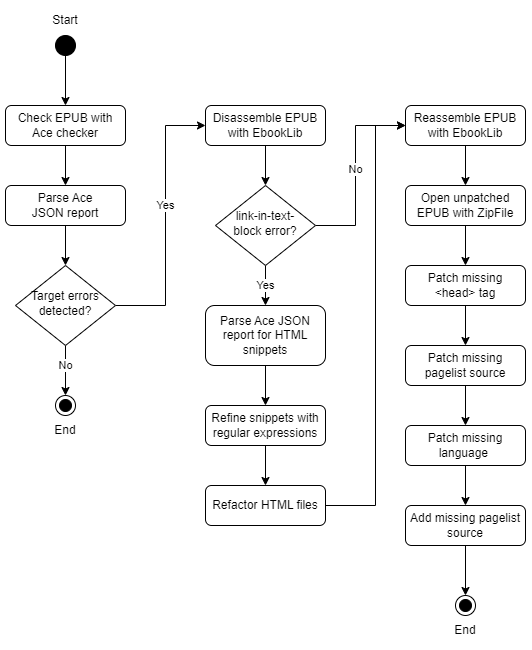
\includegraphics[width=0.48\textwidth,keepaspectratio]{media/images/Flowchart_Methodology_V2.png}
\caption{Process overview of the developed methodology}
\centering
\label{figure:flowchart}
\end{figure}


\subsubsection{Error detection}
To detect the errors that this method addresses, the EPUB is first checked with the Ace checker. The Ace checker generates a JSON and HTML report that represents the assertions of any failed tests. The JSON report is parsed and analyzed to check if any of the three target errors are detected. Depending on the outcome, two booleans (PageBreakFix and LinkFix) are set that dictate which of the respective EPUB fixes are applied. The value of the PageBreakFix boolean is determined by the presence of the \texttt{epub-pagelist-missing-pagebreak} and \texttt{epub-pagelist-broken} errors and the LinkFix value is dependent on whether the \texttt{link-in-text-block} error is found. If neither boolean is set to True, the program closes.


\subsubsection{EPUB preparation}
In the case that an EPUB violates one of the aforementioned rules, the EPUB is loaded into a Python script. This is done with the \texttt{read\_epub()} function from the EbookLib library. The full EPUB data is now held inside an \texttt{EpubBook} object, subsisting of chapters represented as \texttt{EpubHtml} objects, images as \texttt{EpubImage} objects, and other file types as \texttt{EpubItem} objects.


\subsubsection{Error tracing}
Before the \texttt{link-in-text-block} error can be fixed, the specific HTML snippets that cause the error need to be found in the chapters of the EPUB. This is done to alter the source file as little as possible in order to safeguard the integrity of the original author's work. To find the HTML snippets, the JSON report from Ace is loaded which holds the data of the errors. This error data also holds the HTML snippet of the error, denoting its location within the EPUB. For each chapter, this violating snippet of the HTML code is captured in a dictionary datatype. This dictionary now holds all violating snippets per chapter.

After this, the violating snippets are refined further to allow them to match to their respective links in the next step. This is necessary because the HTML snippets generated by the Ace report contain noise making them unable to match to the original HTML code. This rather noisy HTML code from the Ace output can be seen in Figure \ref{figure:aceexample}. The refinement is done by finding the full value of the \texttt{href} attribute using regular expressions. The exact regular expression pattern used for this is: \texttt{href=".*?"}. This results in an organized dictionary with refined HTML snippets that can be used in the next step.


\begin{figure}[h!]
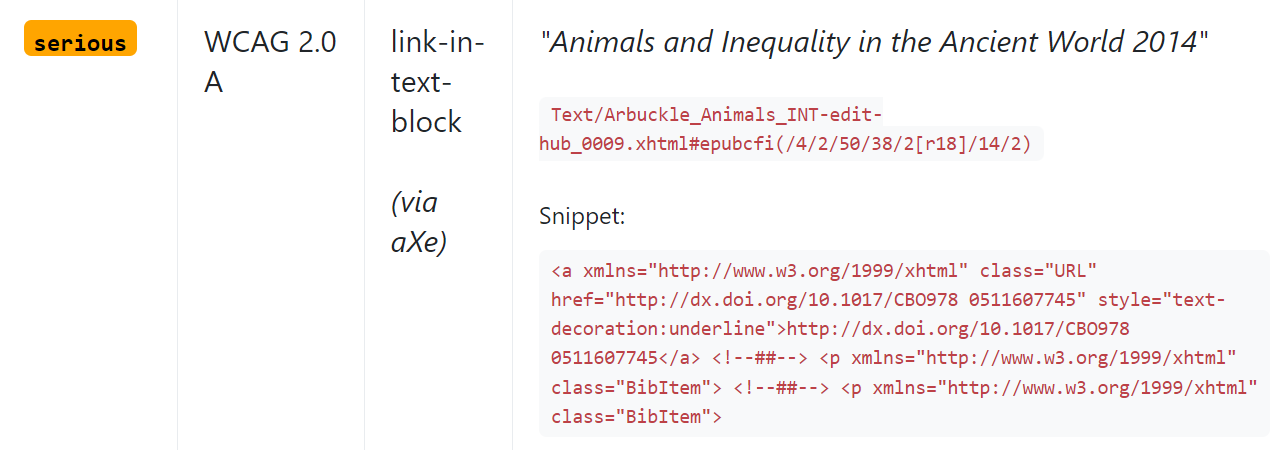
\includegraphics[width=0.48\textwidth,keepaspectratio]{media/images/aceexample.png}
\caption{Example of an Ace \texttt{link-in-text-block} error with an unrefined HTML snippet}
\centering
\label{figure:aceexample}
\end{figure}


\subsubsection{Error fixing}
After the violating HTML snippets have been refined and organized per chapter, the \texttt{link-in-text-block} errors in the EPUB can be fixed. This is done by looping over the HTML files in the EbookLib \texttt{EpubBook} object. Using the \texttt{get\_items\_of\_type
(ebooklib.ITEM\_DOCUMENT)} command, only the HTML files and thus chapters, within the EPUB are targeted. If no violating links are present in a chapter, the chapter can be skipped. However, if violating links are indeed present in the chapter, the HTML snippets are loaded by calling the dictionary. The chapter's content is then parsed with the BS4 library into a 'soup' by using the built-in BS4 'html-parser'.

\begin{figure*}[h!]
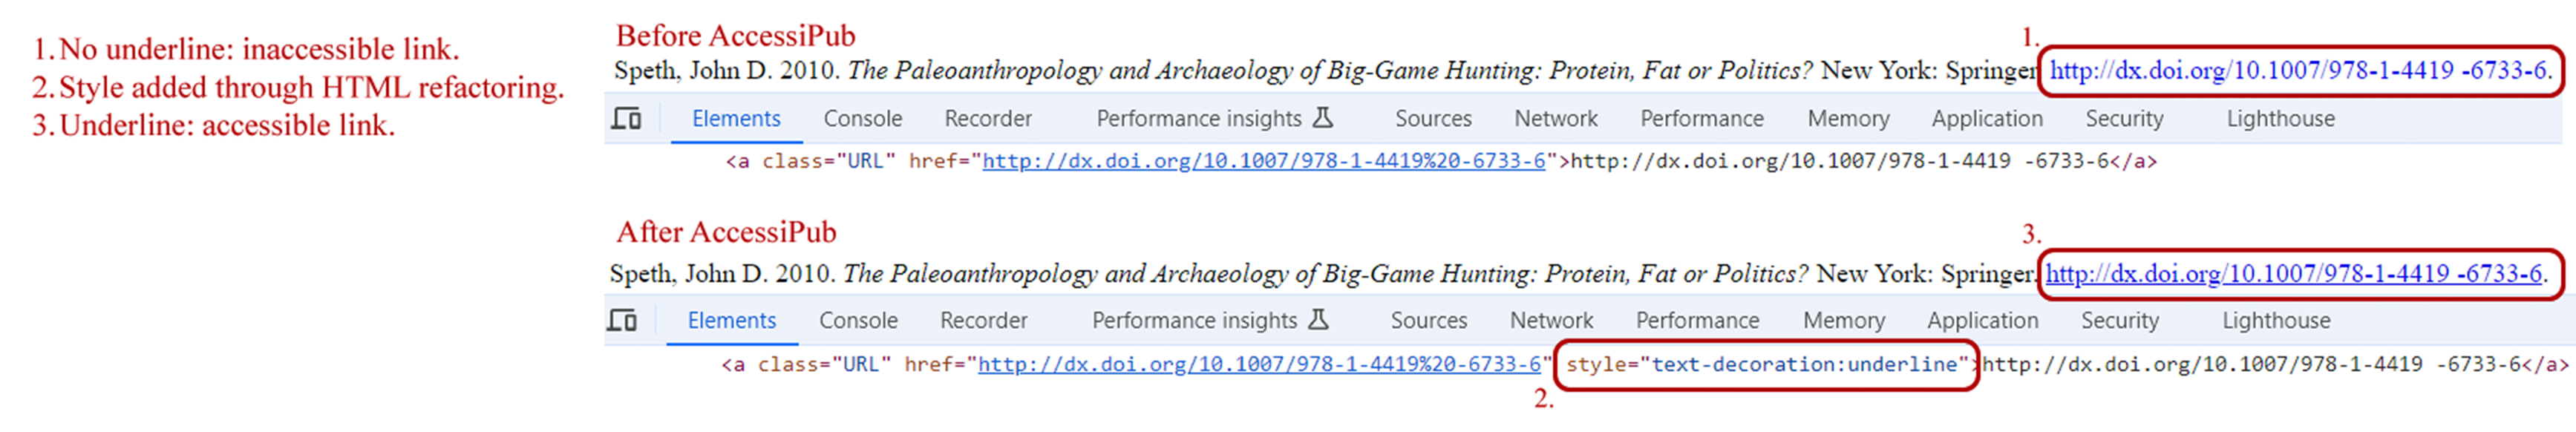
\includegraphics[width=0.96\textwidth,keepaspectratio]{media/images/refactorexample2.png}
\caption{Example of how HTML refactoring directly changes HTML code and improves the accessibility of an EPUB}
\centering
\label{figure:refactorexample}
\end{figure*}

BS4 is used to find all links - represented as \texttt{<a>} tags - in the parsed chapter content by using the \texttt{find\_all()} function, similar to the method of Zhang et al.\cite{Zhang2024}. These links are then looped over and checked if their \texttt{href} attribute is matched with one from the dictionary. If this is the case, it is assigned a \texttt{style} attribute as follows: \texttt{link['style'] = "text-decoration:underline"}. Assigning the value at this level makes sure that the style is applied and visible. Inline HTML styling always takes precedence over styling in the stylesheet, given that the value in the CSS stylesheet does not have the \texttt{!important} tag. In case the \texttt{'text-decoration'} for links is set to 'none' in the stylesheet of the EPUB and contains an \texttt{!important} tag, the tag is removed. This is done with the cssutils library by looping through all style rules and filtering on the aforementioned conditions. Once a style rule is found that matches all conditions, the \texttt{!important} tag is removed.

Following the complete link patch of the HTML content of a chapter, it is converted into a bytestring format using the built-in \texttt{bytes()} function. This is necessary for the EPUB as it also works with bytestrings. This bytestring object is then set as the new content of the \texttt{EpubHtml} object, directly modifying its content, highlighting another strong point of the EbookLib library. All chapters are iterated and patched in this way until the process is complete.


\subsubsection{EPUB reassembling}
After the previous step is completed, the EPUB has to be reassembled. This process is not straightforward, as the EbookLib library is not built to make edits to existing books, but rather to create new books from scratch \cite{EbookLibFAQ}. This limitation causes some hindrances and requires workarounds to make sure that the EPUB is reassembled properly. 
First, a new \texttt{EpubBook} object is created. The title, author, and other metadata are copied over from the original EPUB. All items from the original EPUB are then iterated through. All items that have not been modified are copied over directly to maintain the ebook's integrity. If an item has been modified in the previous step, it is ensured that the modified version is copied over. After this, the original table of contents and spine are copied. The \texttt{EpubNcx()} and \texttt{EpubNav()} functions from EbookLib are then used, as these create the new page-list by using the new modified content. In the case of an \texttt{epub-pagelist-missing-pagebreak} or \texttt{epub-pagelist-broken} error, these functions resolve these errors. The new and updated \texttt{EpubBook} object is now saved to a new EPUB file.

It is important to note in this step that a crucial change was made on line 100 in the utils.py file in the source code of EbookLib. This part of the code is responsible for generating the new page list as part of the \texttt{EpubNcx()} and \texttt{EpubNav()} functions. Previously, this line stated "\texttt{if 'epub:type' in elem.
attrib:}" and has been changed to "\texttt{if elem.get('epub:type') ==
'pagebreak':}". The earlier code only checks if an 'epub:type' is present as an element's attribute. However, this code should be more specific since multiple values for this exist. If the epub:type attribute is set to 'footnote' for example, it should not be included in the page list. The new code makes sure that only page breaks are included in the page list.


\subsubsection{EPUB patching}
This flow unfortunately raises several new errors, mainly caused by limitations in EbookLib mentioned previously. This final step focuses on patching these errors. The tool that is used to accomplish this is the ZipFile module, from the ZipFile library. This library is also able to disassemble an EPUB file, but lacks the powerful functionality that the EbookLib library possesses. This simplicity, however, is what enables the EPUB file to have its elements altered without the errors, caused by EbookLib, to appear again. The newly updated EPUB is loaded into a ZipFile object, allowing it to be looped over in Python.

When reassembling an EPUB with EbookLib, an issue with the library causes it to not include the information stored within the \texttt{<head>} tag \cite{EbookLibHeadTag}. 
This leads to the stylesheet link being lost along with the title, severely altering the appearance of the EPUB. The conceived workaround is to store the information that is inside the \texttt{<head>} tag of the original EPUB. This is added to the new file by looping over all files that end in .xhtml, .html, or .htm. Every file's content is converted to a BS4 object, allowing the \texttt{<head>} tag to be replaced. After, the altered content is converted back into bytes and saved back to the file.

% A similar issue as the above causes the schema

Another issue that plagued EPUBs with a missing page-list is their lack of a reference to a source of the page-list, which is another Ace rule breach and ties in with the EPUB Accessibility standard. The pagination source is stored inside the EPUBs .opf file; the file that hosts most of the metadata of the EPUB. The ZipFile object is looped over to find the .opf file and the content is parsed with BS4. This allows for two \texttt{<meta>} tags and one \texttt{<dc:source>} tag to be added, holding the pagination source information. The pagination source is declared as this thesis' tool name: \textit{AccessiPub}.

Lastly, a large fraction of EPUBs are missing an explicit mention of their language in the .opf file, despite the fact that it's declared in their metadata. If the missing value is detected, the \texttt{xml:lang} attribute is set by taking the language from the EPUB's metadata. This is done during the same step as adding the page source since the BS4 object of the .opf file is already loaded. The BS4 object is converted back to bytes and saved to the .opf file, completing the EPUB patching.

With these additional patches in place, the EPUB is saved to a new file by calling ZipFile's \texttt{close()} function, completing the experimental setup.

\begin{table*}[t!]
% \scriptsize
\begin{center}
\begin{tabular}{ | c || c | c | c |}  
\hline
\textbf{Error type} & \textbf{\#Errors Pre-AccessiPub} & \textbf{\#Errors Post-AccessiPub} & \textbf{\% Change} \\
\hline
link-in-text-block & 620,203 & 14,028 & -97.7\% \\
\hline
epub-pagelist-broken & 31,372 & 0 & -100\% \\
\hline
epub-pagelist-missing-pagebreak & 11,436 & 695 & -93.9\% \\
\hline
\hline
Total target errors & 663,014 & 14,723 & -97.8\% \\
\hline
Total errors & 779,899 & 128,194 & -83.6\% \\
\hline
\end{tabular}
\end{center}
\normalsize
\caption{Target error reduction before and after AccessiPub intervention}
\label{table:targetreduction}
\end{table*}

\subsection{Evaluation}
To evaluate the performance of the methodology, a baseline comparison is conducted. The Ace checker is run before and after the experiment to generate accessibility reports of both states. The following key metrics were taken into account to measure the performance of AccessiPub: total EPUB error reduction, total target error reduction, and relative error reduction per EPUB.
Both the total EPUB error reduction and the total target error reduction were calculated using the following formula, converting the resulting fraction to a percentage. The relative error reduction per EPUB was calculated with the same formula, but applied on a per-EPUB basis.

\[E_{reduction} = \frac{E_{pre AccessiPub} - E_{post AccessiPub}}{E_{pre AccessiPub}}\]


To further solidify the results, a paired t-test was performed to acquire insight into the statistical significance (p < 0.05). The evaluation is conducted on the full OAPEN Foundation dataset and aims to show to what extent the devised methodology reduces accessibility errors in EPUBs.

For this thesis' results, there is no direct comparison possible to other scientific papers, since no other methods exist for improving EPUB accessibility automatically. In order to still put the results of this thesis within the frame of other research, they are compared to the results of papers that improve the accessibility of web pages. In particular, the performance of HTML refactoring on EPUBs is compared to the performance of HTML refactoring on web pages.